\documentclass[12pt, oneside]{article}

%Codificación e idioma
\usepackage[T1]{fontenc}
\usepackage[spanish]{babel}
\usepackage[utf8]{inputenc}

% Url
\usepackage{url}

% Graphics
\usepackage[pdftex]{graphicx}
\DeclareGraphicsExtensions{.png,.jpg}

\usepackage{wrapfig}

%Resaltado de sintaxis
\usepackage{color}
\definecolor{gray97}{gray}{.97}
\definecolor{gray75}{gray}{.75}
\definecolor{gray45}{gray}{.45}

\definecolor{red}{rgb}{0.6,0,0} % strings
\definecolor{green}{rgb}{0.25,0.5,0.35} % comments
\definecolor{purple}{rgb}{0.5,0,0.35} % keywords
\definecolor{blue}{rgb}{0.25,0.35,0.75} % doc

\usepackage{listings}
\lstset {
	language			=	C,
	frame				=	Ltb,
    framerule			=	0pt,
    aboveskip			=	0.5cm,
    framextopmargin		=	3pt,
    framexbottommargin	=	3pt,
    framexleftmargin	=	0.4cm,
    framesep			=	0pt,
    rulesep				=	.4pt,
    backgroundcolor		=	\color{gray97},
    rulesepcolor		=	\color{black},
    %
    stringstyle			=	\color{red},
    showstringspaces	=	false,
    basicstyle			=	\ttfamily\small,
    commentstyle		=	\color{green},
    morecomment         =   [s][\color{blue}]{/*}{*/},
    keywordstyle		=	\color{purple}\bfseries,
    tabsize					=	3,
    %
    numbers				=	left,
    numbersep			=	15pt,
    numberstyle			=	\tiny,
    numberfirstline		=	false,
    breaklines			=	true,
}

\title{Apache Torque}
\author{Francisco J. Serrano}

\begin{document}

\maketitle
\tableofcontents

\section{Introducción}

\subsection{Fundación Apache}

\begin{wrapfigure}{L}{0.3\textwidth}
	
\includegraphics[scale=.8]{img/apache-logo.png}
\end{wrapfigure}

Apache Software Foundation (ASF) es una organización no lucrativa (en concreto, una fundación) creada para dar soporte a los proyectos de software bajo la denominación Apache, incluyendo el popular servidor HTTP Apache. La ASF se formó a partir del llamado Grupo Apache y fue registrada en Delaware (Estados Unidos), en junio de 1999.
Apache Software Foundation es una comunidad descentralizada de desarrolladores que trabajan cada uno en sus propios proyectos de código abierto. Los proyectos Apache se caracterizan por un modelo de desarrollo basado en el consenso y la colaboración y en una licencia de software abierta y pragmática.

\subsection{Apache Torque}

\begin{wrapfigure}{L}{0.4\textwidth}
	
\includegraphics[scale=.8]{img/torque-logo.png}
\end{wrapfigure}

Apache Torque es un mapeador objeto relacional para Java. En otras palabras, Torque te permite acceder y manipular información en una base de datos relacional usando objetos. 
%A diferencia de la mayoría de los otros mapeadores objeto-relacional, Torque no utiliza la reflexión para tener acceso a las clases proporcionadas por el usuario, pero genera las clases necesarias (incluyendo los Objetos) a partir de un esquema XML que describe el diseño de base de datos (que puede ser escrito a mano o generado a partir de una base de datos existente)
El esquema XML puede ser usado para generar y ejecutar un script SQL el cual creará todas la tablas en la base de datos.

As Torque hides database-specific implementation details, Torque makes an application independent of a specific database if no exotic features of the database are used.
Usage of autogeneration eases the customization of the database layer, as you can override the autogenerated methods and thus easily change their behaviour.

\subsubsection{Runtime}
Torque Runtime contiene todo lo necesario para permitir a la aplicación acceder a la base de datos. Es el único componente que Torque necesita en la aplicación y puede ser usado de forma independiente.

\subsubsection{Generator}
Generator contiene las tareas de Ant las cuales hacen todo el trabajo para el plugin Maven. En el caso de usar el plugin Maven, no es necesario usar Generator directamente. No obstante, Generator puede ser llamado directamente desde Ant.

\subsubsection{Ant}

\begin{wrapfigure}{L}{0.3\textwidth}
	
\includegraphics[scale=.9]{img/ant-logo.png}
\end{wrapfigure}

Apache Ant es una libreria de Java y una herramienta de linea de comando cuya misión es
Apache Ant is a Java library and command-line tool whose mission is to drive processes described in build files as targets and extension points dependent upon each other. The main known usage of Ant is the build of Java applications. Ant supplies a number of built-in tasks allowing to compile, assemble, test and run Java applications. Ant can also be used effectively to build non Java applications, for instance C or C++ applications. More generally, Ant can be used to pilot any type of process which can be described in terms of targets and tasks. Ant is written in Java. Users of Ant can develop their own "antlibs" containing Ant tasks and types, and are offered a large number of ready-made commercial or open-source "antlibs". Ant is extremely flexible and does not impose coding conventions or directory layouts to the Java projects which adopt it as a build tool.

\subsubsection{Maven Plugin}

\begin{wrapfigure}{L}{0.3\textwidth}
	
\includegraphics[scale=.8]{img/maven-logo.png}
\end{wrapfigure}

Maven plugin: Apache Maven is a software project management and comprehension tool. Based on the concept of a project object model (POM), Maven can manage a project's build, reporting and documentation from a central piece of information. (Nosotros no lo usaremos)

\subsubsection{Templates}
The templates contain the building blocks used by the generator to create the O/R peer and object classes, SQL scripts and the like. You can change the templates if you want to customize the output of the generator (this is only necessary in very special circumstances). Up to release 3.1.x, the templates were a part of the generator. Starting with the 3.2 release of Torque, the templates have been separated into their own jar archive.

\subsubsection{Village}
Village is a 100\% Pure Java API that sits on top of the JDBC API. El propósito de esta API es hacer mas fácil is to make it easier to interact with a JDBC compliant relational database.

\section{Gestores de bases de datos}

\subsection{Postgresql}

\begin{wrapfigure}{L}{0.3\textwidth}
	
\includegraphics[scale=.8]{img/postgresql-logo.png}
\end{wrapfigure}

PostgreSQL es un sistema de gestión de bases de datos objeto-relacional, distribuido bajo licencia BSD y con su código fuente disponible libremente. Es el sistema de gestión de bases de datos de código abierto más potente del mercado.
PostgreSQL utiliza un modelo cliente/servidor y usa multiprocesos en vez de multihilos para garantizar la estabilidad del sistema. Un fallo en uno de los procesos no afectará el resto y el sistema continuará funcionando.

\subsection{MySQL}

\begin{wrapfigure}{L}{0.35\textwidth}
	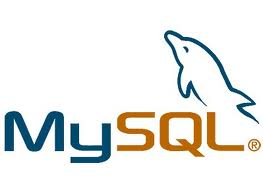
\includegraphics[scale=.3]{img/mysql-logo.jpg}
\end{wrapfigure}

MySQL es un sistema de gestión de base de datos relacional cuya licencia se ofrece bajo GNU GPL.
MySQL usa un sistema multihilo y funciona sobre una gran cantidad de plataformas.
En aplicaciones web hay baja concurrencia en la modificación de datos y en cambio el entorno es intensivo en lectura de datos, lo que hace a MySQL ideal para este tipo de aplicaciones gracias a su motor no transaccional MyISAM.

\subsection{SQL Server}

\section{Instalando Apache Torque}
En primer lugar descargar todo el software necesario:

\begin{description}
	\item[Runtime] \url{http://apache.rediris.es/db/torque/torque-3.3/binaries/torque-3.3.tar.gz}
	\item[Generator] \url{http://ftp.udc.es/apache/db/torque/torque-3.3/binaries/torque-gen-3.3.tar.gz}
	\item[Village] \url{http://apache.rediris.es/db/torque/torque-3.3/binaries/village-3.3.tar.gz}
	\item[Ant] \url{http://ftp.udc.es/apache//ant/binaries/apache-ant-1.8.4-bin.zip}
\end{description}

\subsection{Instalando Ant}
Después de descargar Ant, lo descomprimimos en nuestro directorio C: por ejemplo.
Renombramos la carpeta descomprimida “apache-ant-1.8.4” como “ant”.
Ejecutamos cmd.exe e introducimos las siguientes variables de entorno:

\begin{lstlisting}
ANT_HOME: set ANT_HOME= C:\ant
JAVA_HOME: set JAVA_HOME C:\Program Files\Java\jdk1.7.0_07 (Directorio donde se encuentra vuestra maquina JAVA)
\end{lstlisting}

Introducimos la dirección del directorio “ant” en el PATH:
\begin{lstlisting}
set PATH=%PATH%;%ANT_HOME%\bin
\end{lstlisting}

Obtenemos las dependencias de bibliotecas de Ant:

Desde cmd.exe nos dirigimos al directorio de Ant
Dentro de él ejecutamos los siguiente:  ant -f fetch.xml -Ddest=system

Instalación de Ant finalizada, ya podemos usar Ant desde cmd.exe.

\subsection{Creando un proyecto}
Creamos un nuevo proyecto en eclipse.
En el interior de la carpeta del proyecto descomprimimos los siguientes paquetes: runtime, generator y village.

\subsection{Configurando y ejecutando Generator}
Accedemos a la carpeta “torque-gen-3.3” de nuestro proyecto.

Descargamos el driver JDBC de la base de datos que queremos utilizar, en nuestro caso Postgresql, desde la siguiente dirección: http://jdbc.postgresql.org/ y lo introducimos en la carpeta “lib” de Generator.

En Postgresql, creamos un usuario “user1” con contraseña “user1” y una base de datos llamada “coches”, de la que es propietario “user1”.

Creamos un directorio en la raíz del proyecto llamado “schema”, donde introduciremos el archivo xml en el cual se describe la base de datos.

Editamos el archivo “build.propierties” añadiendo la configuración de nuestro proyecto. En amarillo se encuentran las líneas que han sido modificadas con respecto al archivo de configuración por defecto.

\subsubsection{build.propierties}
El fichero {\bf build.propierties} es un extenso fichero en texto plano estructurado en apartados.

A continuación verá las lineas que han sido necesarias modificar para que el ejemplo {\em coches} funcione correctamente.

En el apartado {\bf PROYECT}, se ha modificado el nombre de proyecto. {\bf Apache Torque} usará {\em el nombre de proyecto} como base tanto para buscar el fichero xml así como nombre base para generar archivos del proyecto.
\begin{lstlisting}
# Nombre de nuestro proyecto
torque.project = coches
\end{lstlisting}

En el apartado {\bf TARGET DATABASE} buscaremos una línea para asignar como valor el nombre de la base de datos que deseemos utilizar. Las opciones disponibles son:

\begin{multicols}{2}
\begin{itemize}
	\item axion
	\item cloudscape
	\item db2
	\item db2400
	\item hypersonic
	\item interbase
	\item msaccess
	\item mssql
	\item mysql
	\item oracle
	\item postgresql
	\item sapdb
	\item sybase
\end{itemize}
\end{multicols}

En nuestro ejemplo usuaremos {\bf PostgreSQL}, por lo que la variable quedaría definida:
\begin{lstlisting}
# Gestor de bases de datos que vamos a usar
torque.database = postgresql
\end{lstlisting}

En el apartado {\bf DATABASE SETTINGS}, configuraremos las opciones de conexión del JDBC. Estos datos son usados por {\bf Ant} para inicializar el sistema Torque con el SQL generado.
\begin{lstlisting}
# Direcciones de acceso a la base de datos y puerto de escucha
torque.database.createUrl = jdbc:postgresql://127.0.0.1:5432/coches
torque.database.buildUrl = jdbc:postgresql://127.0.0.1:5432/coches
torque.database.url = jdbc:postgresql://127.0.0.1:5432/coches

# Driver para acceder a la base de datos
torque.database.driver = org.postgresql.Driver

# Usuario y password para acceder a la base de datos
torque.database.user = user1
torque.database.password = user1

#Direccion del host donde se encuentra la base de datos
torque.database.host = 127.0.0.1

# Direccion donde se generaran los ficheros .java y .sql
torque.output.dir = ../src

# Direccion desde donde se obtendra el esquema .xml de la base de datos
torque.schema.dir = ../schema
\end{lstlisting}

\subsection{Configuración}
\subsection{Compilando nuestro primer proyecto}
\subsection{Configuración XML}
	\begin{center}
		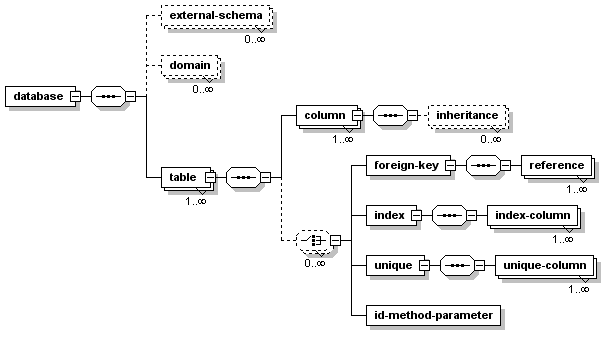
\includegraphics[height=8cm]{img/xml-config.png}
	\end{center}

\section{Uso de Apache Torque}

\section{Aplicacion}
\subsection{Esquema base datos}
\begin{lstlisting}[language=xml]
<!DOCTYPE database SYSTEM
 "http://db.apache.org/torque/dtd/database_3_3.dtd">

<database name="notas">
  <table name="usuario" description="Tabla de usuarios">
    <column
      name="usuario_id"
      required="true"
      primaryKey="true"
      type="INTEGER"
      description="Identificador de usuario"/>
    <column
      name="nick"
      required="true"
      type="VARCHAR"
      size="128"
      description="nick del usuario"/>
  </table>
  <table name="nota" description="Tabla de notas">
    <column
      name="nota_id"
      required="true"
      primaryKey="true"
      type="INTEGER"
      description="Identificador de nota"/>
    <column
      name="texto"
      required="true"
      type="VARCHAR"
      size="150"
      description="texto de la nota"/>
	<column
      name="usuario_id"
      required="true"
      type="INTEGER"
      description="Clave foranea de usuario"/>
	<foreign-key foreignTable="usuario">
      <reference
        local="usuario_id"
        foreign="usuario_id"/>
    </foreign-key>
  </table>
</database>
\end{lstlisting}

\end{document}